\documentclass{standalone}
\usepackage{pgfplots}
\pgfplotsset{compat=1.8}

\begin{document}
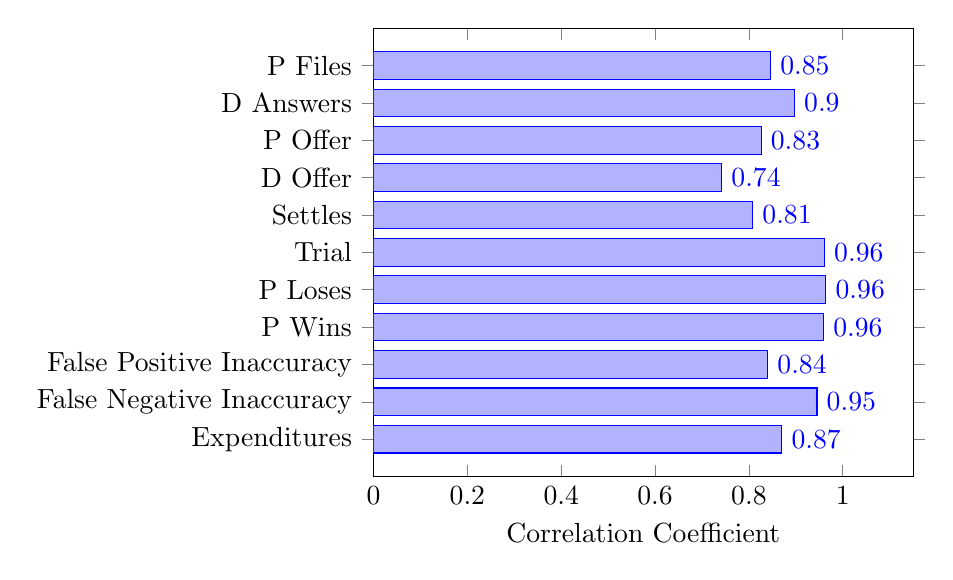
\begin{tikzpicture}
\begin{axis}[ 
xbar, xmin=0, xmax=1.15,
xlabel={Correlation Coefficient},
symbolic y coords={
	{Expenditures},
	{False Negative Inaccuracy},
	{False Positive Inaccuracy},
	{P Wins},
	{P Loses},
    {Trial},
    {Settles},
    {D Offer},
    {P Offer},
    {D Answers},
    {P Files},
    },
ytick=data,
nodes near coords, 
nodes near coords align={horizontal},
ytick=data,
]
\addplot coordinates {
    (0.846,{P Files}) 
    (0.897,{D Answers}) 
    (0.826,{P Offer}) 
    (0.742,{D Offer}) 
    (0.808,{Settles})
    (0.961,{Trial}) 
    (0.964,{P Loses}) 
    (0.959,{P Wins}) 
    (0.840,{False Positive Inaccuracy}) 
    (0.945,{False Negative Inaccuracy}) 
    (0.870,{Expenditures}) 
    };
\end{axis}
\end{tikzpicture} %width=6cm,height=7.59cm
\end{document}